\section{Traction surface loading}

The application of surface loading by specified traction involves computation
of the term
\begin{displaymath}
\Pi_{ext} = \int_{\Gamma_t} \delta \B{u} \, \bar{\B{T}} \, \dif \Gamma
\end{displaymath}
for cases where the traction $\bar{\B{T}}$ is specified on the reference
configuration.
For cases in which the traction is specified on the deformed configuration
the loading is obtained from
\begin{displaymath}
\Pi_{ext} = \int_{\gamma_t} \delta \B{u} \, \bar{\B{t}} \, \dif \gamma
\end{displaymath}
and then often also requires computation of a tangent term.

At present \textsl{FEAP} includes only the first option for some special cases.

\subsection{\texttt{NSURface} loading}

The \texttt{NSURface} loading option is restricted to normal loading applied
to \textit{straight} edges of two dimensional \texttt{NPATch} region.
The can be specified by a linear or quadratic Lagrange interpolation between
specified end points.  For linear variation the data is given as
\begin{verbatim}
       NSURface
         SIDE LINEar nside
           1  x1  y1 p1
           2  x2  y2 p2
\end{verbatim}
and for quadratic variation by
\begin{verbatim}
       NSURface
         SIDE QUADratic nside
           1  x1  y1 p1
           2  x2  y2 p2
           3  x3  y3 p3
\end{verbatim}
where \texttt{x3, y3} is an intermediate point between \texttt{x1, y1}
and \texttt{x2, y2}.  The parameter \texttt{side} refers to a specific
\texttt{NSIDe} number.

\subsection{\texttt{NLOAd} patch loading}

\begin{figure}[b!]
\begin{center}

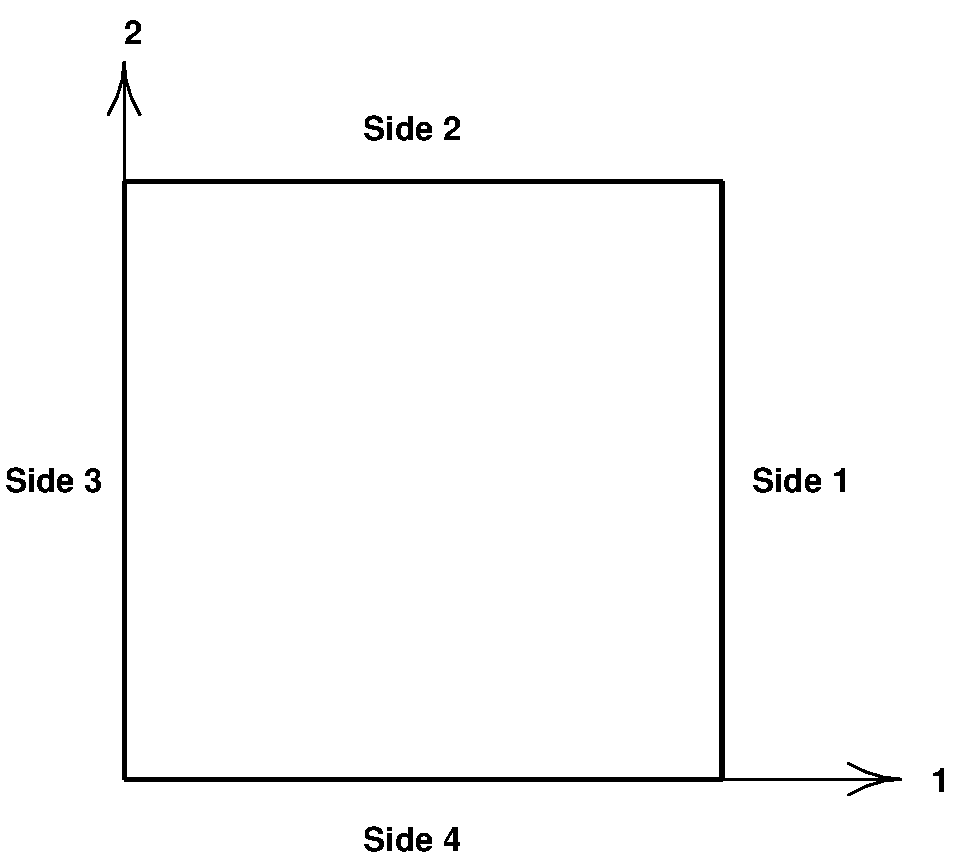
\includegraphics[height=3in]{figs/nside2d}

\caption{Side designation for a two dimensional NURBS patch. \label{fig3a} }
\end{center}
\end{figure}

The  \texttt{NLOAd} option permits a constant traction loading to be
specified on
any face of a two or three dimensional \texttt{NPATch}. Table \ref{tab2.1}
indicates how faces are numbered on patches.
For two dimensional patches the side numbers also are denoted as shown in
Figure \ref{fig3a} where the $1$ and $2$ directions are associated with the
knot directions.

This option produces \textit{dead} loading only (\textit{i.e.}, loads associated
with the reference configuration). The advantage over use of \texttt{PRESsure}
material sets (see Sect. \ref{pressure}) results from only one computation to
compute effective control point forces. Whereas, loads from the pressure
set are computed for each iteration in the solution by integration over the
affected surface.  Pressure set loading, however, can be computed on the
current configuration as follower type loads.

\begin{table}[h]
\begin{center}
\begin{tabular}{|c || r | r |} \hline
Face & \multicolumn{1}{c|}{2 Dimensions} & \multicolumn{1}{c|}{3 Dimensions} \\ \hline
1 & +1 knot & +1 knot \\
2 & +2 knot & +2 knot \\
3 & -1 knot & +3 knot \\
4 & -2 knot & -1 knot \\
5 & -- & -2 knot \\
6 & -- & -3 knot \\ \hline
\end{tabular}
\caption{Face numbers for \texttt{NPATch} patches. \label{tab2.1} }
\end{center}
\end{table}

Three options for loading direction are available: \texttt{NORMal},
\texttt{TRACtion} and \texttt{USER}.  The \texttt{USER} option requires
the addition of a user prepared subprogram, although a sample is available
for uniform tension in the $x_1$ coordinate direction of an infinite domain
containing a circular hole of radius $R$.
For the \texttt{NORMal} option the data is specified as
\begin{verbatim}
       NLOAd
         NORMal patch face pressure prop-num
\end{verbatim}
where \texttt{patch} is the number of the \texttt{NPATch}; \texttt{face} is the
face number on the patch; \texttt{pressure} is the normal traction acting
on the face and \texttt{prop-num} is a proportional load number for time
dependent loading.

For the \texttt{TRACtion} option the data is specified as
\begin{verbatim}
       NLOAd
         TRACtion patch face traction direction prop-num
\end{verbatim}
where \texttt{traction} is the intensity of the specified traction;
\texttt{direction} the global direction of application and \texttt{prop-num}
is a proportional load number for time dependent loading.

For the \texttt{USER} option the data is specified as
\begin{verbatim}
       NLOAd
         USER patch face value-1 value-2 prop-num
\end{verbatim}
where \texttt{value-1} and \texttt{value-2} are two user available parameters
and \texttt{prop-num} is a proportional load number for time dependent loading.
